\chapter{PBTC System Design}

The following chapter discusses design decisions and justifications of PBTC and the developed simulation tool. The outcomes discussed in this chapter are:

\begin{itemize}
\item design of an appropriate model of individual vehicle priority,
\item design of a phase control algorithm, to be operated on a 2 phase intersection,
\item evaluation methodology and relevant measures of effectiveness used to compare the performance of a developed PBTC system to existing alternatives.
\end{itemize}

\section{Priority Modeling}

Representative modeling of the priority of vehicles and passengers approaching an intersection is required to effectively design, develop and evaluate the PBTC system within a realistic setting. 

The priority of an individual vehicle is proportional the cost, measured in cents, of stopping and/or delaying the vehicle at a PBTC controlled intersection. A single cost figure is calculated by an aggregation of the current effective delay cost, potential stopping cost, and potential delay cost for the vehicle. The operational stopping cost calculation is based on the velocity, acceleration, mass, and engine efficiency of a vehicle. Delay cost is based upon the class of vehicle, an individual notion of urgency, and number of passengers.

Emphasis has been placed on approximations of cost components that can be calculated efficiently in real-time by a traffic light controller. In order to develop realistic approximations of cost components, the following assumptions have been made about the physical characteristics of vehicles and driver behaviours:

% list of the high level assumptions here 
\begin{itemize}
\item vehicles are classed as light or heavy, with petrol and diesel engines respectively,
\item vehicle mass, engine efficiency, and aerodynamic properties are considered constant per vehicle class. Table ~\ref{vehicleclassconstants} shows the constants representing the physical properties of each vehicle class,
\item the price per litre for petrol fuel is \$2.24, and diesel fuel \$1.65 (New Zealand Dollars), based upon market values at the time of writing.
\end{itemize}

\begin{table}[H]
\centering
\renewcommand{\arraystretch}{1.25}
 	
	\begin{tabular}{@{}lrr@{}} \toprule
		Quantity & value for light vehicles & value for heavy vehicles \\ \midrule
		Mass & 1,500kg & 15,000kg \\
		Engine efficiency factor & 0.3 & 0.3 \\
		Fuel type & petrol & diesel \\
		Fuel price & \$2.24\text{/l} & \$1.65\text{/l} \\
		Fuel energy density & 3.6x10^6 \text{J/l} & 3.6x10^6 \text{J/l} \\ \bottomrule
	\end{tabular}
	
	\caption{ Physical vehicle constants per vehicle class used as parameters for the physics based consumption model. Light vehicles are cars only, heavy vehicles can be buses or trucks within the PBTC system. }
	\label{vehicleclassconstants}
\end{table}

% subsections discussing the design of each measure here:

\subsection{Operational Stopping Cost}

The operational stopping cost of an individual vehicle is the economic cost expended whenever the vehicle is delayed or forced to stop at a controlled intersection. The stopping cost of a vehicle is proportional to the cruise speed of the vehicle before the stop, and recognises that a vehicle that has been forced to stop expends a certain amount of fuel after takeoff in order to reach the speed of travel before stopping. Calculating an estimation for the cost of stopping a vehicle involves estimating the number of litres of fuel consumed when decelerating and accelerating at a controlled intersection.

Modern cars are typically capable of calculating and displaying the instantaneous or cumulative fuel consumption for a journey. \citeasnoun{kesting2013traffic} present a method for calculating fuel consumption as a function of driving resistance and velocity using a physics based consumption model. This instantaneous fuel consumption model was used in simulation as part of a priority message from a vehicle upstream of a traffic signal controller, however it was found that the fuel consumption rate alone is not appropriate for estimating the operational stopping cost of a vehicle, as it is dependent on vehicle speed and acceleration at the instant of communication.

Models exist for retrospective analysis of fuel consumption over a journey, using measured speed and acceleration rates over time and could be used to find the total cost of a stopping and accelerating through a controlled intersection after a vehicle has completed a trip (Akcelik & Besley, 2003; Treiber & Kesting, 2013; Treiber, et al., 2008). Attempts to im- plement these models at various time steps to estimate consumption leaving an intersection were not successful at producing meaningful results as an assumed arbitrary rate of predicted acceleration is not appropriate for all vehicles and speed limits. In practice, driver behaviour, vehicle characteristics, and intersection geometrics are likely to significantly de- crease the accuracy of a predictive acceleration estimation.

An alternative appropriate measure of operational stopping cost is achieved by the PBTC system through a physics-based consumption model considering the deceleration and acceleration stages of a stop for a particular vehicle. As most modern car engines employ fuel cutoff during deceleration to prevent unnecessary fuel use, the total fuel used can be approximated solely on the acceleration component of a stop at an intersection \cite{kesting2013traffic}. 

The PBTC system estimates the fuel consumption of a vehicle departing an intersection by calculating the kinetic energy of the vehicle before the stop. By making an assumption that the vehicle will accelerate to their previous approach speed when leaving the intersection, the calculation is a reflection of how much energy is lost if the vehicle is requested to stop as it will require at least this much energy to reach the approach speed of the vehicle before the stop. This assumption does not hold in all circumstances, for example whenever downstream links of an intersection are heavily saturated with slow moving traffic, however it is a reasonable estimation for free flowing traffic as the approach and departure speeds are likely to be equal to the speed limit of the area. 

Given the kinetic energy of an approaching vehicle is known, the litres of fuel required to generate this energy can be found based on the calorimetric energy density of the fuel being burned by the engine and the mechanical efficiency factor of the vehicle engine. Equation ~\ref{fuelconsump} summarises the calculation of the operational stopping cost based on this method.

% equation here
\begin{align}
	\centering
		\text{operational stopping cost} &= {{\text{change in kinetic energy} \over {\text{engine efficiency} \times \text{calorimetric fuel density}}}} \times \text {fuel price per litre} \\ 
		& = {\frac{\frac{1}{2}m{v}^{2} }{c\substack{d} \times w\substack{cal}}} \times {p_\text{f} \text { / L}}
	\label{fuelconsump}
\end{align}

This physics based consumption model is only an approximation of the actual fuel consumption of approaching vehicles, but appropriately differentiates between light and heavy vehicles. More sophisticated estimations of fuel consumption would be desirable in practice and could be achieved through reinforcement learning using accurate measures of fuel consumption communicated by a vehicle to a traffic controller after it has departed an intersection.

% rephrase/move to stopping cost section
%While accurate measurements for the stopping cost and journey fuel consumption can be made after a vehicle has passed through an intersection, it is not possible to produce an accurate model for estimating fuel consumption for each approaching vehicle as speed and acceleration and as a result fuel consumption, is dependent not only on the physical characteristics of the vehicle and driver behaviour, but also the speed and acceleration of surrounding vehicles. 

\subsection{Delay Cost}

The delay cost of a vehicle approaching a traffic light is dependent on the urgency of travel of the vehicle occupants. Delay costs for a vehicle occupant can be defined proportional to the "lateness" of a passenger to reach a given destination by a predetermined time. For example, if a passenger is travelling from Wellington CBD to the airport and has only 10 minutes available before check-in closes for a flight, the cost of delay of the journey should reflect the money the passenger will effectively lose if they miss the flight and must rebook tickets or cancel their trip.

The calculation of a delay cost for each vehicle requires user input of the urgency of travel for a passenger or passengers. This project assumes vehicles on the road network are equipped with a dashboard computer with capability of inputting any required variables. A number of alternative variables of user input have been considered during development of the PBTC system, including arrival time and relative urgency. 

In an arrival time based approach, a user would be required to set their destination and desired time of arrival into the dashboard computer, to be sent to a PBTC traffic controller when approaching an intersection. The PBTC controller can estimate the travel time to the destination and based on the arrival time, assign a cost of delay to the vehicle. One of the advantages of this method is that a sophisticated network of connected PBTC controllers could share knowledge of traffic conditions at each intersection and calculate an accurate measure of the likely travel time based on a route to the destination. Extensions to such a system could also calculate and inform a driver of the best route to the destination based on the passenger urgency, i.e., routing all low priority drivers to a more congested route and redirecting high urgency vehicles to a faster alternative. A significant disadvantage of this approach is the higher complexity of input by a user. If a user does not know the travel time to a destination from their current location, they may inadvertently allocate themselves maximum urgency by setting a short time of arrival and as a result it is more difficult for the system to consider a range of vehicle urgencies.

As an alternative, a relative urgency measure is used by the PBTC system, which asks a driver to set their own perceived urgency as a discrete integer on a scale from one to five. This measure is both easy for vehicle occupants to understand, and simple for a PBTC controller to consider the urgency of an individual vehicle relative to others at an intersection. Passengers can use their knowledge of the approximate travel time to a destination and importance of the journey to make their own judgement about urgency of passage at an intersection. A potential drawback of this system is the ease of which it can be abused, for example all drivers can easily set their urgency to the maximum value. This project assumes that this does not happen, and in practice the higher price payed to pass an intersection at a higher urgency will prevent this behaviour. 

For simplicity, the PBTC system assumes that all passengers in a vehicle have identical urgency and as a result, the  delay cost is linearly proportional to the number of passengers in a  vehicle. Consequently, vehicles with higher passenger occupancy are favoured by the PBTC system, encouraging more efficient use of road networks through ride-sharing or carpooling initiatives. Reducing the number of single occupant vehicles on our roads reduces congestion and fuel emissions, and shares the costs of maintaining and running a vehicle between multiple individuals and is similarly encouraged by High Occupancy Vehicle (HOV) lanes in use on modern highways with congestion problems.

The economic cost of delay to the vehicle occupants is calculated using the NZTA's estimated average figure of \$26.20NZD per vehicle hour (cite here).The PBTC system makes the assumption that this figure is representative of the cost of delay for an average journey, and hence reflects a single-occupant vehicle with an urgency of 3. Assuming $t$ as the time a vehicle is delayed in seconds, $u$ as the discrete relative urgency input by the vehicle occupant/s, and $p$ as the number of passengers in a vehicle, a formula for the overall cost of delaying a vehicle, $c_\text{d}$, is given as

% equation here
\begin{equation}
	c_\text{d} &= t ^{s(u)} * 0.007(\frac{u}{3}) * p 
	\label{delaycostequation}
\end{equation}

Where 0.007 is the delay cost in cents per second, and $s(u)$ is a constant for each vehicle class, determined by
% equation here
\begin{equation}
	s(u) = \left\{
	      \begin{array}{lr}
	     	1 & : u \leq 3\\
	         1.1  & : u = 4 \\
	         1.25 & : u = 5
	     \end{array}
	   \right.
	\label{delayslopeequation}
\end{equation}

Figure ~\ref{delaycosturgency} shows the relationship between delay cost and time delayed for each of the five discrete urgency values for up to sixty seconds of delay. 

For simplicity, the PBTC system assumes all urgency values are constant and do not change during the time a vehicle is waiting at an intersection. In a real-world system this model is likely to be too simplistic. Depending on the initial urgency of the vehicle, as the length of time that vehicle has been delayed increases, their urgency to pass the intersection will also increase and the costs of delay will compound. There is also a limit to this relationship, for example, if the occupants of a vehicle are delayed to the point that they miss their meeting, flight, or other appointment, their urgency may reduce significantly and/or they may change destination and return home. Modeling these cases was not determined to be relevant within the simulation environment. 

\begin{figure}[]
\centering
	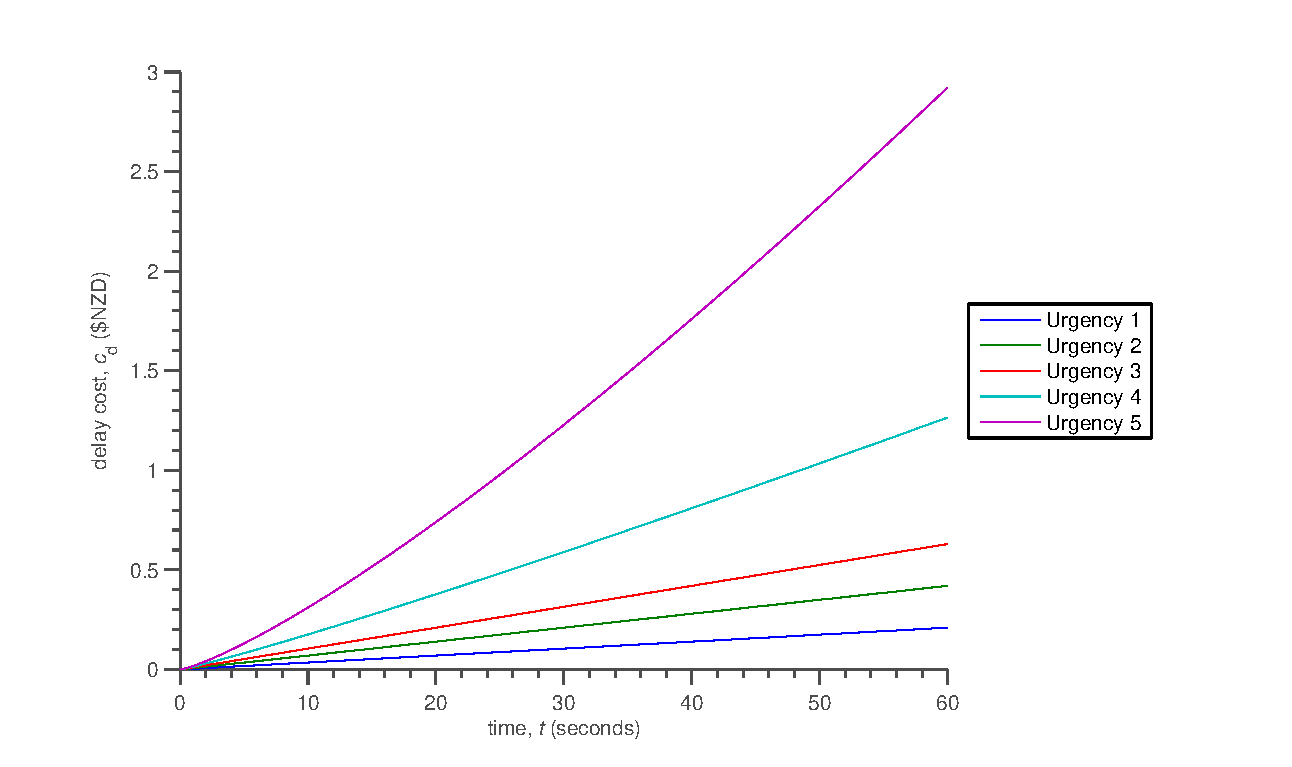
\includegraphics[scale=0.65]{delay_cost_per_urgency.eps}
	\caption{Cost of delay per time for a range of occupant urgency values, from time of zero seconds up to sixty seconds. }
\label{delaycosturgency}
\end{figure}

\section{PBTC System Design}

% the PBTC controller seeks to improve on existing delay or saturation based method by including the costs of travel for each vehicle in the control algorithm decision
 \citeasnoun{kesting2013traffic} describes the `Golden Rule of Traffic Flow Optimisation` as trying to homogenise traffic flow with respect to time, spatial arrangement, and local speed differences.

\subsection{Assumptions}

Design of a system for producing an optimal, minimal cost solution to phase assignment at any arbitrary controlled intersection is a difficult problem and evaluating such a system requires a sophisticated simulator capable of realistically modeling real world intersection geometrics, driver behaviours, and traffic flows. Development of these capabilities for simulation is an effort beyond the scope of this project. For this reason, the following assumptions have been made to simplify development of the PBTC control algorithm within this project:

\begin{itemize}
\item the control algorithm operates over a two-phase intersection, with each phase allocating green to one of two flows of traffic approaching the intersection only,
\item approaching vehicles represent straight through demand for the intersection only, no left/right split phases (i.e "arrow lights") are required,
\item the algorithm is limited to a single, isolated intersection only and does not consider any aspects of coordination between neighbouring intersection controllers.
\end{itemize}

\subsection{Vehicle-Controller Communication}

Communication between approaching or waiting vehicles and a PBTC controller at an intersection is required to provide inputs to the control algorithm to make a cost effective choice of phase timings based on the real-time traffic conditions. The implementation details of the required communication network is beyond the scope of this project and suggested as an area for future research. This project assumes that all of the necessary technology required for vehicles to send small packets of information to a controller exists in every vehicle using the road network, and each vehicle sends its own state information directly to the roadside intersection controller.

In the simulation developed as part of this project, vehicles approaching or waiting a PBTC controlled intersection broadcast their current state to the intersection controller every two seconds if the distance to the intersection stop line is less than 150 metres. There are two justifications for this behaviour, firstly; although in a simulated environment any object can feasibly read the properties of any other object at any time, it is important to consider the real world application of the system where network latency and limited network capacity are real problems that prevent instantaneous, real-time messaging with no delay. 

Secondly, consider a situation where a single vehicle is approaching a red light at an intersection where there is no demand for the competing green phase; in a stop-line actuated control system the vehicle will be forced to stop, wait at least six seconds for the lights to react and change phase, and then take off. By allowing a 150 metre broadcast window, a PBTC controller is able to respond to this situation and change the phase before the approaching vehicle has reached the lights, preventing them from stopping. The 150 metre window is based on assuming an approaching vehicle is traveling at a constant speed below 80km/h (approximately 22 m/s), requiring at least 133 metres of clearance given a typical controller requires 6 seconds of inter-green time to change a phase. In practice, it might be useful to be able to tweak the distance at which cars would be considered by the PBTC system based on the speed limit of the area. 

\begin{figure}[]
\centering
	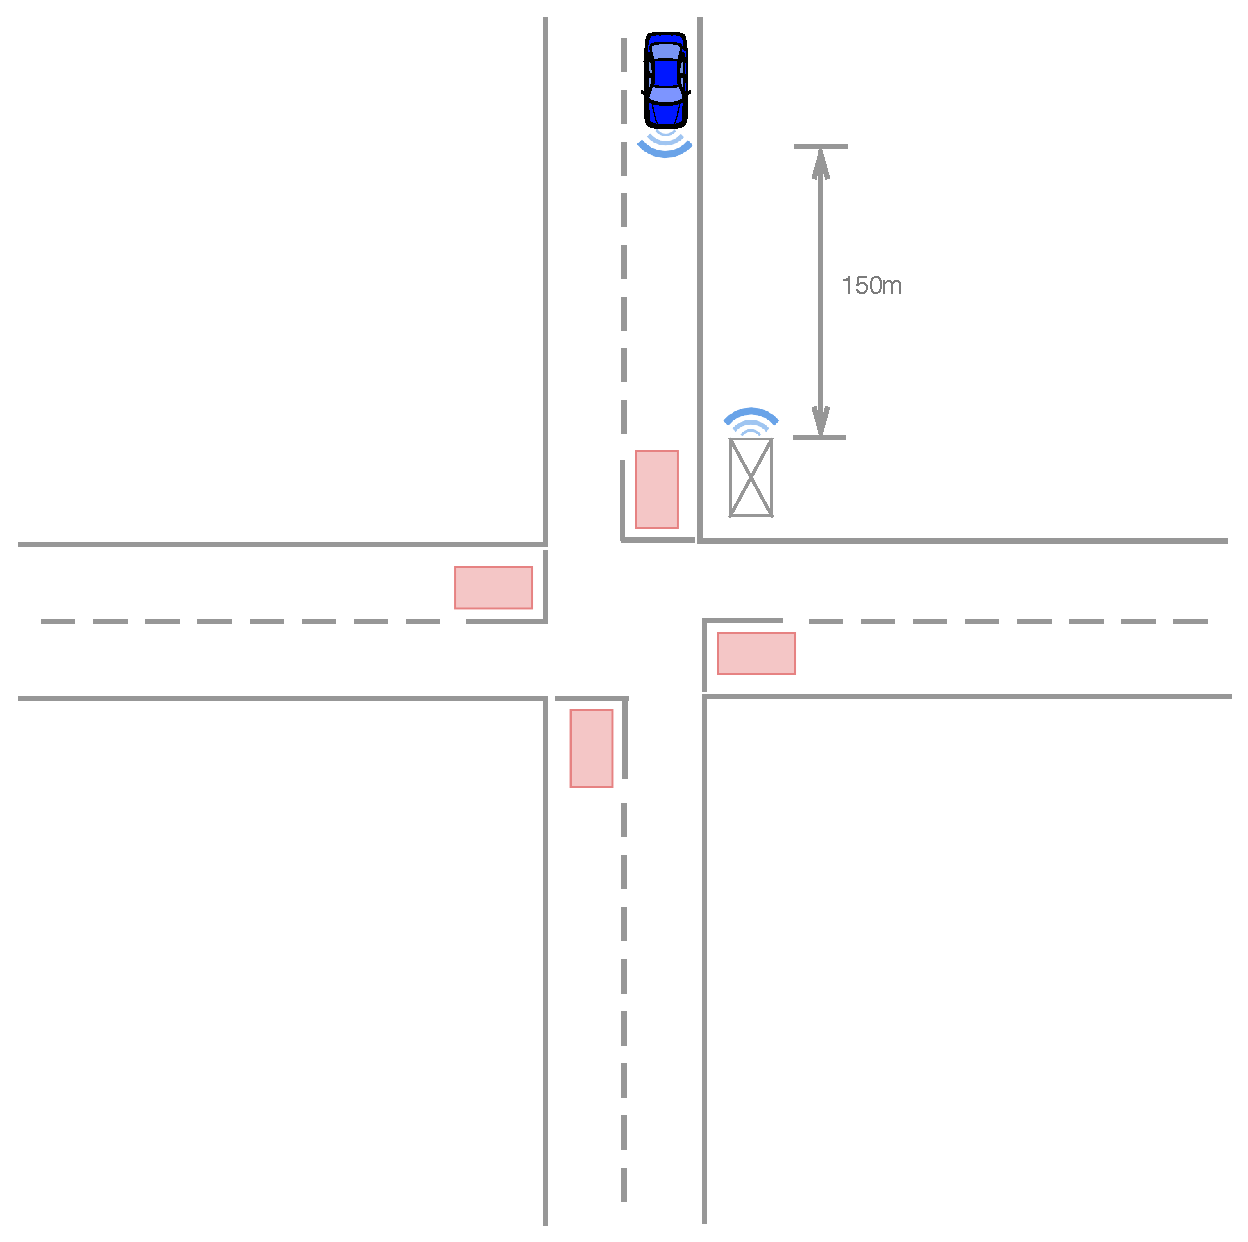
\includegraphics[scale=0.5]{intersection_diagram.eps}
	\caption{ Plan elevation of a simple four way intersection showing an approaching vehicle communicating with a PBTC controller. The distance of initial communication is shown as 150 metres. The position of stop-line detectors typically used by SCATS systems are shown in red. The PBTC controller is able to adapt to vehicle actuations in advance of the vehicle arrival at the stop line. }
\label{intersectiondiagram}
\end{figure}

\subsection {Control Algorithm Design}
\label{sec:PBTCDesign}

The PBTC control algorithm is a primary component of the PBTC system, designed to be executed by a roadside traffic controller to determine which phases should operate, the order of operation, and duration of each phase; in real-time. The primary objective of the PBTC control algorithm is to reduce the total economic cost incurred by vehicle movements  at PBTC controlled intersection, using traffic composition information communicated to a controller by vehicles in the network. 

Phases of an intersection are preconfigured based upon the geometry of the intersection. Each phase within the PBTC system contains an allocation of green or red signals to each light at a controlled intersection, such that no two competing traffic flows receive a green light at the same time in a phase. Two traffic flows are said to be competing if a collision would occur if vehicles on each flow entered the intersection at the same time. Each phase also defines a minimum time the phase must run for.  The minimum time condition is a safety consideration of the system, designed to allow enough time for at least one vehicle to pass safely through the intersection before the phase is changed. 

The order and duration of phases at a PBTC controlled intersection is determined by calculating aggregate costs of delay and operation for each approach of an intersection. A PBTC controller maintains a list of messages received from approaching or delayed vehicles that are used for calculation of the delay costs and operational stopping costs for each vehicle and aggregated to find the total costs for an approach. 

% primary cost of changing phase is the operational cost of stopping and delaying free flowing traffic
The primary cost of changing phases at a controlled intersection is the cost of stopping and delaying free flowing traffic. As a result, the standard operation for a PBTC controlled intersection is to run a set phase continuously until a phase change is determined to be cost effective and scheduled by the PBTC control algorithm. This behaviour is designed to produce minimal changes to the system, effectively maximising the homogeneity of free flowing traffic until the cost of interfering becomes low relative to the cost of doing nothing. 

A phase change is scheduled by a PBTC controller if the sum of the cost of stopping the traffic flow currently approaching a green signal, defined as the phase change cost or $c_\text{pc}$, is less than the total incurred cost of delay for all vehicles queued and waiting at any approaches displaying a red signal, defined as the phase delay cost or $c_\text{pd}$. The cost of stopping the traffic flow on a green signal also includes an estimation of the potential delay cost for each vehicle assuming they must be delayed \emph{at least} as long as the minimum condition for the newly scheduled phase. Equations X and X define the phase change cost and phase delay cost in a mathematical notation. 

\begin{equation}
	c_\text{pc} &= \sum_{v \in approaches.green.vehicles} c_\text{stop} + c_\text{delay(min)}
	\label{phaseChangeCostEq}
\end{equation}

\begin{equation}
	c_\text{pd} &= \sum_{approach \in approaches.red} \sum_{v \in approach.vehicles} c_\text{stop} + c_\text{delay(min)}
	\label{phaseDelayCostEq}
\end{equation}

If this condition is true at any time, the algorithm enters a phase change sequence. During a phase change sequence, a lookahead heuristic is applied to find the minimum potential cost incurred as a result of the change. Based on a predefined lookahead table size, the controller estimates the total cost of changing phase for each second from zero up to the table size, constructing a table with each row representing a time in seconds and the cost of stopping the phase at that time. The controller then dynamically extends the current phase duration by the number of seconds that corresponds with the lowest cost value in the lookahead table.

The lookahead method used in the PBTC control algorithm is an optimisation method performing a local search for a time of changing phases that incurs the least cost to the system. For example, consider an intersection where two vehicles have been waiting at a red signal for 60 seconds, and the cost of delay has exceeded the cost of stopping the opposing traffic flow receiving a green signal. If two vehicles are approaching the intersection on the freely flowing approach but are close enough to stop if the phase is changed immediately, the cost of the change includes the operational cost of stopping the two vehicles and the cost of delaying the vehicles for the minimum duration of the next phase. 

Due to their distance from the intersection and current velocity, after one additional second the two moving vehicles may pass through the intersection and these costs are avoided, with the trade-off cost being one more second of delay for the two waiting vehicles. Unless the two waiting vehicles have high urgency and a high number of passengers, the cost of an additional second of delay is likely to be marginal. The lookahead procedure of the PBTC control algorithm will evaluate the total cost of extending the current phase by a fixed number of seconds to allow the moving vehicles to pass, and extend the current phase by the calculated minimum time if it is found to be less than the cost of an immediate change.

\begin{algorithm}[H]
 \SetAlgoLined
 \KwData{
 	c_p: current phase, n_p: next scheduled phase, a: set of approaches, K: lookahead window size
 }
 \KwResult{ minimal cost time until phase should be change executed }
 \Begin{
  set $totalStoppingCost$ = 0 \; \\
  set $totalDelayCost$ = 0 \; \\
  \For{approach in approaches}{
  	\If{approach signal is red} {
		add cost of delay for all vehicles queued on approach to $totalDelayCost$ \;
	} 
	\Else{
		add cost of stopping and cost of minimum delay for all vehicles on approach to $totalStoppingCost$ \;
	}
  }
  \If {$stoppingCost < delayCost$} {
  	set lookaheadTable = [] \;
	\For{$i := 0$ to K} {
		lookaheadTable[i] = cost of delay for all stopped approaches over $i$ + cost of stopping for all vehicles that cannot clear the intersection after $i$ seconds \;
	}

  set extendedGreenTime = index of minimum value in lookaheadTable \;	
  return extendedGreenTime \;
}
return -1 \;	 \tcc*[r]{no change scheduled}
 }
 \caption{PBTC phase scheduling algorithm}
\end{algorithm}

% discuss lookahead search tree from other paper here

\section{Evaluation Methodology}

Performance evaluation and analysis is required to determine the effectiveness and appropriateness of the PBTC system. Performance evaluation of traffic control methodology is made difficult by the proprietary and commercial nature of traffic control algorithms and the software systems that implement them. All New Zealand intersections are controlled by the SCATS system, which is commercially developed in Australia and in use in many countries worldwide. No test bed or performance evaluation software is available for SCATS, and as a result a direct comparison with the SCATS implementation is not possible.

An alternative to a direct comparison with the SCATS system considered during the development of this project was to develop a simplified and approximate system that was based off the methodology of SCATS. While this method had the advantage of being able to produce a flexible estimation system that can be easily benchmarked against the PBTC system, there are disadvantages related to implementing an approximation to be representative of the real system. 

Firstly, there is a very limited amount of publicly accessible information related to the design and implementation of the SCATS control algorithms. One of the very few papers available described some algorithms of the very first version of the SCATS system \citeasnoun{lowrie1982scats}, however it is not easy to know how much the system has improved since this paper was published. Secondly, it is not easy to determine how good of an approximation any simplified implementation of SCATS would be without being able to benchmark against the real system leading to potentially inaccurate comparisons. 

As a result of these two limitations of developing a custom, simplified SCATS implementation, the evaluation component of this project was designed based on using reports generated by SCATS containing phase times and traffic conditions of the SCATS system operating on intersections in Wellington over a 12 hour period. The reports used during evaluation were generously provided by the Wellington City Council (WCC), who operate SCATS for all of the intersections in the central Wellington City area. 

SCATS allows WCC engineers to produce reports showing data and intersection state information for every cycle of operation, including exact phase times and the number of vehicle detections per phase. The evaluation component of this project was designed to use the information contained within these reports to reconstruct a realistic representation of SCATS operation in Wellington. This method was preferred over the custom implementation of SCATS because of the relative ease of generating vehicle arrivals and scheduling phase times based off the SCATS reports in simulation. As a result, this method of evaluation the closest to an accurate representation of the real SCATS behaviour, and is easily evaluated over an extended period of operation. 

The 12 hour period of operation was determined with consideration to the typical profile of traffic in the central Wellington City area during a day. A typical day for an inner city intersection is characterised by two "peaks" of traffic congestion in the morning and evening for around 1-2 hours each. Traffic composition around these peaks typically consists of motorists on a morning or evening commute to and from inner city offices for work. By evaluating traffic performance over a 12 hour period from 7AM to 7PM, these peaks can be included in the evaluation, creating a range of traffic conditions for performance analysis. 

%The primary goal of the PBTC system is to reduce the economic costs of delay at a controlled intersection and as a result, evaluation metrics discussed here are designed to measure the impacted costs of running the system over an extended period of time for an intersection.







